\section{Architecture}
The \graphioli \gls{framework} realizes the \gls{MVC} design pattern in which the classes are separated by their function in either `Model', `View' and `Controller'.\par
This is achieved by the following design:\par

\begin{description}
	\item[Model] The model contains the \ref{cls:gameboard} that serves as a mediator between the logical \gls{graph} (\ref{cls:graph}) and the visual graph on a \gls{grid} (\ref{cls:grid}).
	\item[View] An implementation of the \gls{interface} \ref{cls:view} is responsible for output and capturing user interactions.
	\item[Controller] The controller is divided into three parts. \ref{cls:gamemanager} conducts the basic game operations and interacts extensively with the class that inherits from \ref{cls:game} (not part of the framework). The \ref{cls:viewmanager} maintains consistency with the \emph{View}.
\end{description}

\begin{figure}[h]
	\centering
	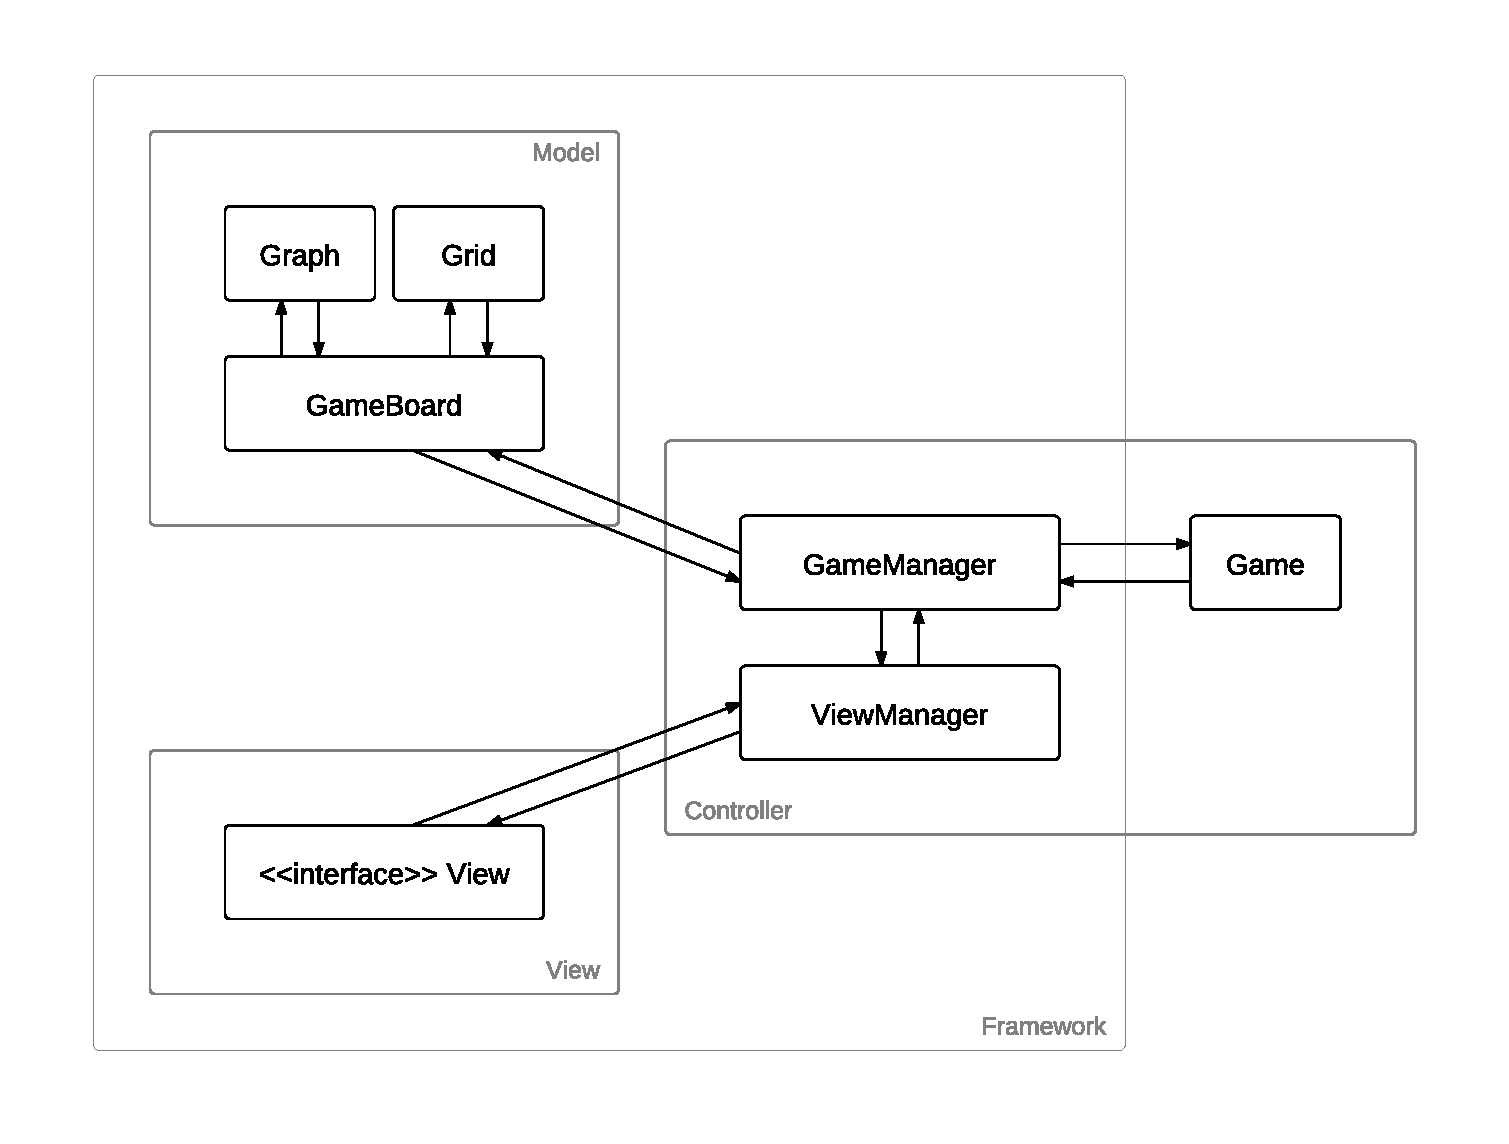
\includegraphics[width=1\textwidth]{archMVC.pdf}
	\caption{Diagram showing the realization of the \gls{MVC} design pattern by the framework.}
	\label{img:archMVC}
\end{figure}